%!TEX root = draft_v2.tex
\section{Complexity}\label{sec:complexity}
The computational complexity of the considered algorithm can easily be bounded. In order to give implementation
free bounds we specify only floating point operations (flops). For each given active set the solver has
to solve at most $2N$ mpQPs, which is done by decomposing the problem as stated in section~\ref{sec:gen:mpQP},
in the worst case this requires one QR decomposition, with $\frac{4}{3}n^3$ flops, and one Cholesky decomposition,
with $\frac{n^3}{3}$ flops, where $n$ is the number of optimisation variables. Solving the worst case problem
on one stage therefore requires $\frac{5}{3}(2n_x^3+n_u^3)$ flops, in the worst case $N$ stages need to be solved,
so that the worst case computational burden for the solution of the mpQP sequence is given 
by~$\frac{5N}{3}(2n_x^3+n_u^3)$. To the authors' best knowledge there are no sensible bounds on the number of
active set changes, so that no bound can be given on the number of times the sequence has to be solved.
In section~\ref{sec:example} we state the case of an example system with an implementation in MATLAB.


\section{Example}\label{sec:example}
In this section we present a numerical simulation for a simplified levitating ball model, as derived in 
by~\cite{Schaich:2015}. The dynamics of the nonlinear system are given $m\ddot y = m g - c\frac{i^2}{y^2}$,
where $m$ denotes the mass of the ball, $g$ denotes the gravitation constant, $c$ denotes a constant depending
on the coil, $y$ the vertical distance to the coil, the simplification is due to neglecting inductive dynamics 
and assuming we that can influence the current~$i$ directly. Figure~\ref{fig:levitating:ball} illustrates the setup.
Choosing the state $x=(y,\dot y)$ and the input $u=i$ we obtain a state space representation which depends nonlinearly
on both the state and the input. An equilibrium is given for all $u=\sqrt{\frac{gm}{c}}x_1$.

Linearising the nonlinear differential 
equation $\dot x = f(x,u)$ around an equilibrium point $(\hat x, \hat
u)$ gives the approximate linear model 
%
\[
	 \Delta\dot{x} = \underbrace{\left(\begin{array}{cc}
	0 & 1 \\ \frac{2c\hat u^2}{m\hat x_1^3} & 0
	\end{array}\right)}_{\frac{\partial f}{\partial x}(\hat x,\hat
      u)}\Delta x 
+ \underbrace{\left(\begin{array}{c}
	0 \\ - \frac{2c\hat u}{m\hat x_1^2}
	\end{array}\right)}_{\frac{\partial f}{\partial u}(\hat x,\hat
      u)}\Delta u
\]
%
where $\Delta u = u -\hat{u}$ and $\Delta x \approx x-\hat{x}$.
We derive the discrete time dynamics with sampling rate $T_s$ using
the Euler formula $x^+=x+T_s f(x,u) =:\tilde f(x,u)$ giving
\[
\Delta x^+ = A \Delta x + B \Delta u , \quad
\Biggl\{\begin{aligned} A &= I+T_s\frac{\partial f}{\partial  x}(\hat
  x,\hat u) \\
B &= T_s \frac{\partial f}{\partial u}(\hat x,\hat u)
\end{aligned}
\]
%
A representation of the form~\eqref{eq:the:problem} can be obtained by sampling input and state
constraints and using the mean-value theorem, as elaborated by~\cite{Schaich:2015}. This leads
to a disturbance representation of the form $\mathcal W(x,u)=\{w\in\mathbb R^n: 
\min_{k\in\mathcal S_w}\{ H_{k,i}^x x + H_{k,i}^u u\} \leq w_i \leq \max_{k\in\mathcal S_w} 
\{ H_{k,i}^x x + H_{k,i}^u u \} \}$,
where ${k\in\mathcal S_w}$ denotes the sample index and $i$ the row number. This point-wise polytopic representation
in addition with a polyhedral representation of state constraints allows us to compute a polyhedral
MRPI set~$\mathcal X^\infty$. As a terminal feedback controller $K$ we use the solution to the robust 
Lyapunov condition $V(x)-V((A+BK)x+Dw)\leq \gamma^2 w^Tw$ 
with $V(x)=x^T P_0 x\geq0$, i.e. $x^TP_0x - ((A+BK)x+Dw)^TP_0((A+BK)x+Dw)\geq x^T(Q+K^TRK)x -\gamma^2 w^T w$, 
see e.g.~\cite{Boyd:94}. This semi-definite program also returns a value for $\gamma^2$. Starting from 
a polyhedral MRPI set~$\mathcal X^\infty$ we apply the algorithm presented in section~\ref{sec:preliminaries}
to obtain the necessary stage constraints~$\mathcal Z_k$. At this stage we can introduce numerical values
for individual parameters, we use $T_s=30ms, C=1\frac{kg m^3}{A^2s^2}, m=100g, \hat x_1 = 50mm$ and $\mathcal X=\{x:
\abs{x_1- \hat x_1}\leq 1mm\wedge \abs{x_2}\leq 105\frac{mm}{s}\}$, $\mathcal U=\{u:\abs{ u-\hat u}\leq10mA\}$.
To obtain $\mathcal W(x,u)$ we sample $\mathcal X$ and $\mathcal U$ with a total of 25 samples, i.e. the cardinality
of $\mathcal S_w$ is 10. In the simulation we use horizon length $N=5$. We perform a cold started line search from $\chi_0=(0,0)$
to the outer bound of the constraint set at $\chi_e=(1,-30)$, the resulting trajectories at the boundaries of
individual active sets are plotted in figure~\ref{fig:plot}.

The simulation was implemented in MATLAB only using non optimised in-built functions for the main computational
purposes. In the simulation illustrated in figure~\ref{fig:plot} there were a total of 10 iterations required,
out of which 7 correspond to changes of the dominating right hand side of $\mathcal W(x,u)$, for which no recomputation
of the solution is necessary. Performing the entire linesearch to the boundary of the feasible set took $0.3765s$.

\begin{figure}
\centering
% \begin{overpic}[scale=0.75]{levitatingBall}
% \put(30,5){$m g$}
% \put(30,41){$c\frac{i^2}{x^2}$}
% \put(78,28){$y$}
% \put(90,89){$i$}
% \end{overpic}
\begin{lpic}{levitatingBall(.75,)}
\lbl[tr]{25,3; $m g$}
\lbl[br]{25,25; $c\frac{i^2}{y^2}$}
\lbl[bl]{49,17; $y$}
\lbl[bl]{56,55; $i$}
\end{lpic}
\vspace{-2mm}
\caption{Levitating ball system.}
\label{fig:levitating:ball}
\end{figure}

\begin{figure}
\centering
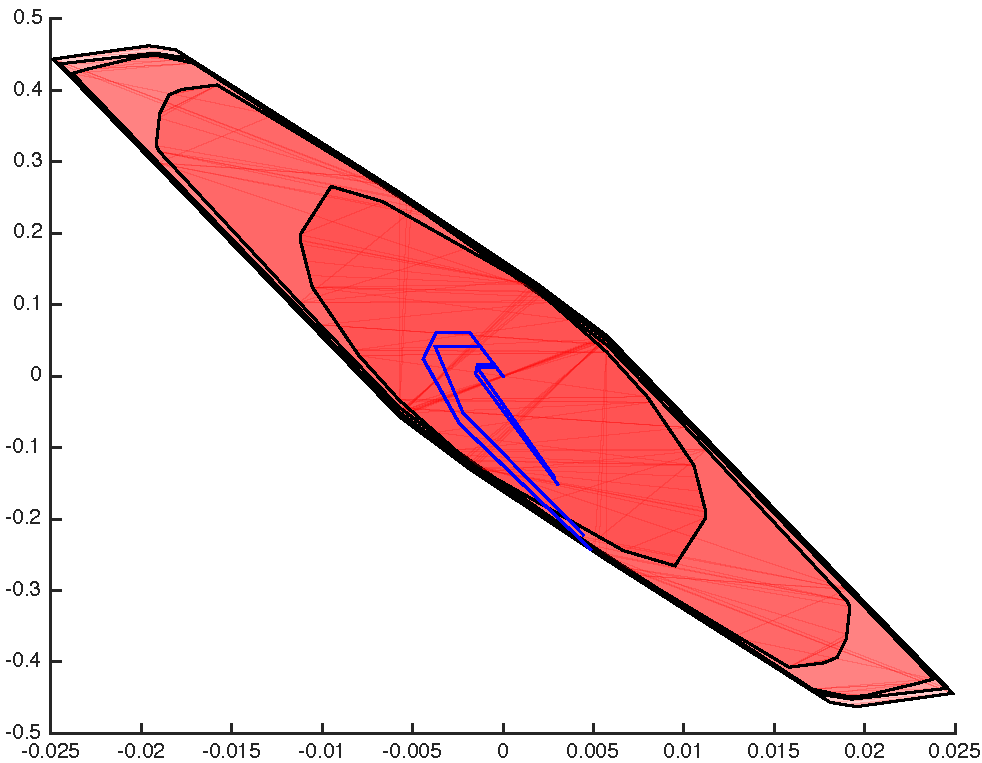
\includegraphics[width=\columnwidth]{myplot}
\caption{Projected stage constraints $\mathcal X_i, i=1,\dots,N$ in red. Trajectories
at the active set changes and on the boundary in blue.}
\label{fig:plot}
\end{figure}

% This section we present a numerical simulation in which the state-dependent uncertainty enters through an upper bound on the linearisation
% error for a nonlinear system. We consider an inverted pendulum described by $ml^2\ddot\varphi = mlg\sin\varphi+M$, where
% $m=0.1$\,kg is the mass, $l=0.3$\,m is the length of the pendulum, $g=9.81$\,m\,s$\mbox{}^{-2}$ is the gravitational
% constant and $M$ is the direct torque input. Discretisation using Euler backward finite differences 
% at $f = 20$\,Hz yields
% \begin{equation}
%   \begin{split}
%     x_1[k+1] &= x_1[k] + \frac{1}{f} x_2[k]\\
%     x_2[k+1] &= \frac{g}{fl} \sin(x_1[k]) + x_2[k] + \frac{1}{fml^2}u[k]
%   \end{split}
% \end{equation}
% where $x_1[k] = \varphi(t_0+k/f),x_2[k] = \dot\varphi(t_0+k/f)$ and $u[k] = M(t_0+k/f)$.
% The nonlinearity is given by the sine function, and we can explicitly state the 
% linearisation error as $e(x_1)=\frac{g}{fl}(\sin x_1 - x_1)$. Since the linearisation
% only approximates the nonlinear dynamics around the equilibrium we can choose a closed interval 
% $0\in D\subset\mathbb R$ and maximise the upper bound 
% \begin{equation}
%   \Delta e = \max_{x_1\in D}\abs{\frac{de}{dx_1}} = \frac{g}{fl}\max_{x_1\in D}\abs{\cos x_1-1}.
% \end{equation}
% This results in the linear system
% \begin{equation}
%   x^+ = \underbrace{\left(\begin{array}{cc}
%   1 & f^{-1}\\ g(fl)^{-1} & 1
%   \end{array}\right)}_A x + \underbrace{\left(\begin{array}{c} 0 \\(ml^2f)^{-1} \end{array}\right)}_B u
%   +\left(\begin{array}{c}w_1\\ w_2\end{array}\right)
% \end{equation}
% with $\abs{w_1}\leq w_{1,\max}$ and $\abs{w_2}\leq\max\{w_{2,\max},\Delta e \abs{x_1}\}$.
% We also introduce the input constraint $\abs{u}\leq3$\,N\,m and use the interval $D = [-\frac{3\pi}{4},
% \frac{3\pi}{4}]$ and a horizon of $N=7$ to obtain the sequence of state constraints $\mathcal X_m$
% depicted in Figure~\ref{fig:numerical:example}. The line search starting at the origin and
% exploring towards $\mathpzc x_e=(-6,50)$ produces the optimal trajectories at the active-set switches
% which are illustrated in blue. In pink a warm-started line search terminates on the boundary of the
% feasible set before reaching the (infeasible) state $\mathpzc x_e=(0,30)$.